\section{Detailed project description}



\subsection{Architectural Design}\label{sec:arch}

\todo{Vorschlag: Architectural Design nennen und vieles kürzen}

\app's basic architecture consists of the following parts:

\begin{itemize}
\item The smartphone, including a NFC chip as well as an internet connection to register with the service.
An internet connection is only be needed once during initialization of the system or when creating a new key pair in case of revocation.
The smartphone must be able to create an asymmetric key pair and securely store it persistently.
\item The Door Access System, also including a NFC chip which can send and receive.
A simple NFC reader would not suffice as it would be vulnerable to replay attacks.
The door system needs access an intranet in order to check if the student/employee has access to the specific area and to get other information for realizing security features like encryption of the communication.
Therefore, some kind of computer is needed, interacting with the NFC hardware as well as with the backend.
\item A backend system, which checks student ID, the corresponding TUMOnline token and fetches the generated public key from the smartphone.
It finally stores the public key of every registered student.
At every door access attempt it checks the TUM active directory if the person is still a student.
\item The TUMOnline system, which provides a secure way to confirm that a user is real.
This is done via a token that the user has to activate in TUMOnline.
\item The TUM active directory (AD), which has enrolment information about every student and can confirm the status of a person.
\end{itemize} 
The last two items are important for the understanding of the whole solution. They were of course already existing and were not altered for this project.\todo{bis hier sollte es jetzt passen}

\bigskip

Figure \ref{fig:arch_ov} gives a holistic overview of the basic architecture (based on public-key cryptography as discussed in section \ref{sec:alt:proto:pubkey}\todo{brauchen wir die Klammer hier?}):
\begin{figure}
\centering
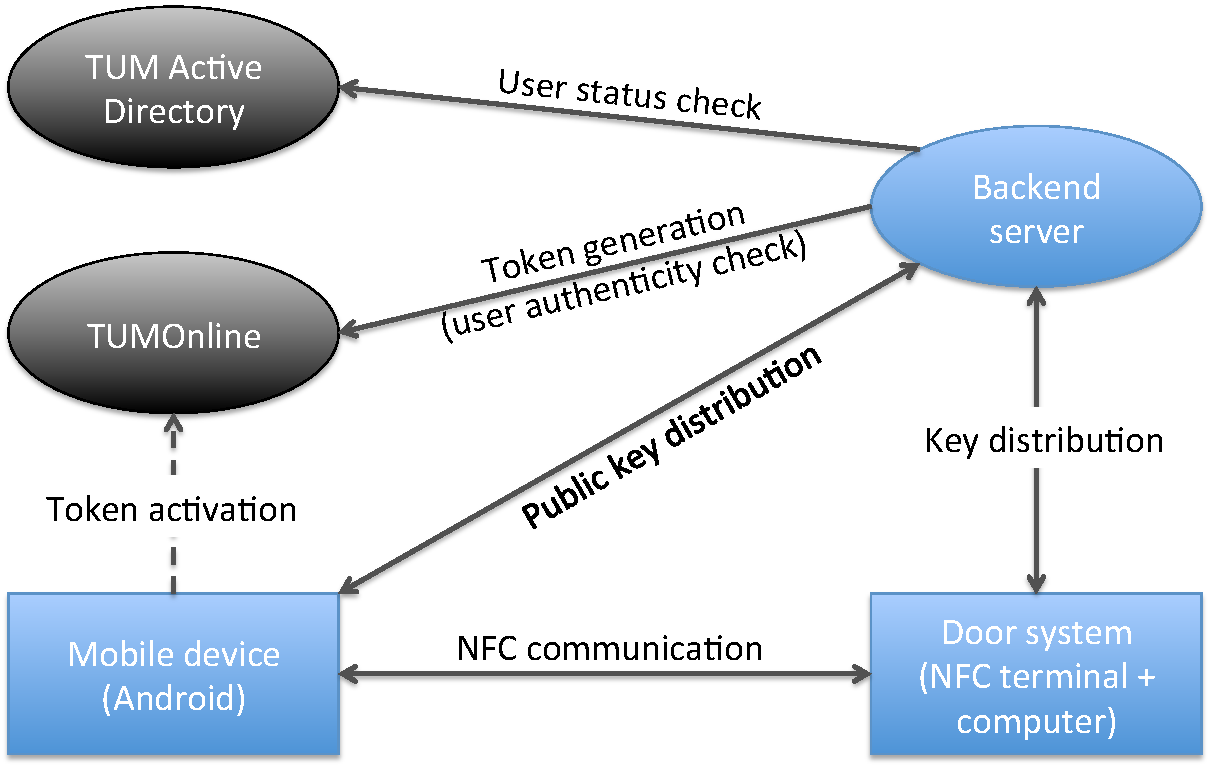
\includegraphics[width=0.8\textwidth]{basic_arch}
\caption{Architectural overview of the \app solution.}
\label{fig:arch_ov}
\end{figure}

\subsection{Registration with Back-end}
To initialize the system, the user has to contact the back-end system once for authentication.
% by providing his user ID.
The user provides his ID along with the user token that is generated by TUMOnline.
%To activate the user token that is generated by TUMOnline, the user has to login separately on a web platform. 
The back-end system can check if the proposed access token of the user is valid or not via the TUMOnline Webservice API.
%For that purpose, the connection to the TUMOnline service is needed to get this kind of information.
If the user has sent the right access token, the back-end system will demand the public part of the user's asymmetric key pair (which has been created on the user's smartphone before starting the communication).
In this step, the server will take particular care that the authentic user is in possession of the private part of the transmitted public key and doesn't pretend to be a different identity.
%create a public key pair and will send the user his private key. Therefore, a key storage and management system has to be implemented.
All connections to the back-end are planned to be secured by TLS.


\subsection{Authentication between Smartphone and NFC Transceiver}
After the user has registered with the back-end system, he can communicate with the NFC reader. 
A three-way handshake assures a secure connection between smartphone and NFC reader.
In order to verify the soundness of the procedure, in particular the authenticity of the communication partner, the NFC reader (i.e.~the system behind it) will fetch the public key of the user who wants to authenticate from the back-end system.
Furthermore, the Door Access System will check if the user has access to the requested area.
It will finally unlock the door if all checks were positive.
